\documentclass[11pt, a4paper]{article}
\usepackage[utf8]{inputenc}
\usepackage[a4paper, margin=2.5cm, top=20mm, bottom=22mm]{geometry}
\usepackage{listings}
\usepackage[english]{babel}
\usepackage{fancyhdr}
\usepackage[%  
    colorlinks=true,
    pdfborder={0 0 0},
    linkcolor=blue
]{hyperref}
%\lstset{language=C,keywordstyle={\bfseries \color{black}}}
\usepackage{subcaption}
\usepackage{graphicx}
\usepackage{caption}
\captionsetup[figure]{font=small}
\captionsetup[subfigure]{font=small}
\captionsetup[table]{font=small}
\usepackage{cleveref}


\setlength\parindent{0pt}

\pagestyle{fancy}
\fancyhf{}
\rhead{Tydings Morrison McClary}
\lhead{Statistical Methods - Assignment 2}
\cfoot{\thepage}



\title{%
    \textbf{Statistical Methods - Assignment 2} \\
    \large Social, Cognitive, and Affective Neuroscience\\
    %Freie Universität Berlin, FB Erziehungswissenschaften und Psychologie\\
    SoSe 2021}

\author{Tydings Morrison McClary \\
    Matrikelnr.: 5133472}
\date{Deadline: August $ 15^{th} $, 2021}

\begin{document}

\null  % Empty line
\nointerlineskip  % No skip for prev line
\vfill
\let\snewpage \newpage
\let\newpage \relax
\maketitle
\let \newpage \snewpage
\vfill
\thispagestyle{empty}
\break % page break
%\maketitle


\newpage
\section*{\centering \underline{Problem 1}}

Before running analysis on the data, the \emph{rest} condition was removed from all four participants and the \verb|NiftiMasker| function from \verb|nilearn| was used for run-wise detrending, standardising, masking, smoothing (Gaussian kernel with 4mm FHWM), and high-pass filtering with a cutoff frequency of $\frac{1}{128}$Hz.\\

\noindent
\textbf{a)} A pipeline was created for both the logistic regression (LR) and support vector classification (SVC) models that included additional standardizing and feature selection using the \verb|sklearn| functions \verb|StandardScaler| and \verb|SelectKBest| with 1500 features to retain for training the model. Comparing the performance of a multinomial LR with a linear SVC using three different multiclass classification strategies implemented in \verb|sklearn| (OneVsOne (OVO) and OneVsRest (OVR) from the \verb|sklearn.multiclass| module as well as the OneVsRest strategy inherent to both classifiers) and a leave-one-run-out cross validation showed that for both classifiers the inherent OneVsRest strategy performed best (Fig.\ref{fig:all_acc}). Furthermore, the LR model outperformed the linear SVC in both OVR settings (Fig.\ref{fig:tot_acc_ovr},\ref{fig:tot_acc}). In general, both models with the inherent OVR were able to decode better for subjects 1 and 2 (Fig.\ref{fig:ind_acc}).
%\begin{figure}[hbt!]
%    \centering
%\end{figure}
\begin{figure}[hbt!]
    \centering
        \begin{subfigure}[b]{0.49\linewidth}
        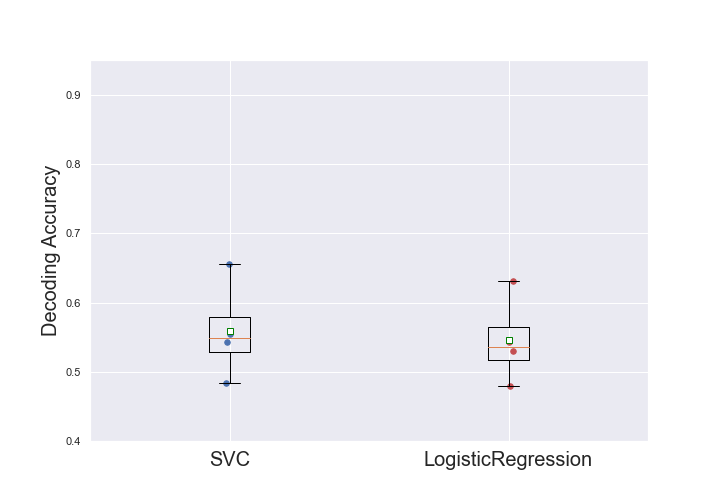
\includegraphics[width=\linewidth, height=6cm]{acc_tot_OVO.png}
        \caption{Total Accuracy for OVO}
        \label{fig:tot_acc_ovo}
        \end{subfigure}
        \begin{subfigure}[b]{0.49\linewidth}
        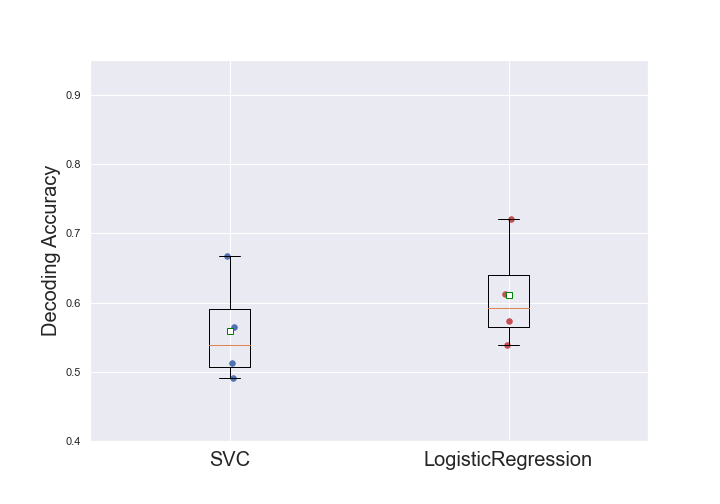
\includegraphics[width=\linewidth, height=6cm]{acc_tot_OVR.png}
        \caption{Total Accuracy for OVR}
        \label{fig:tot_acc_ovr}
        \end{subfigure}
    	\begin{subfigure}[b]{0.49\linewidth}
        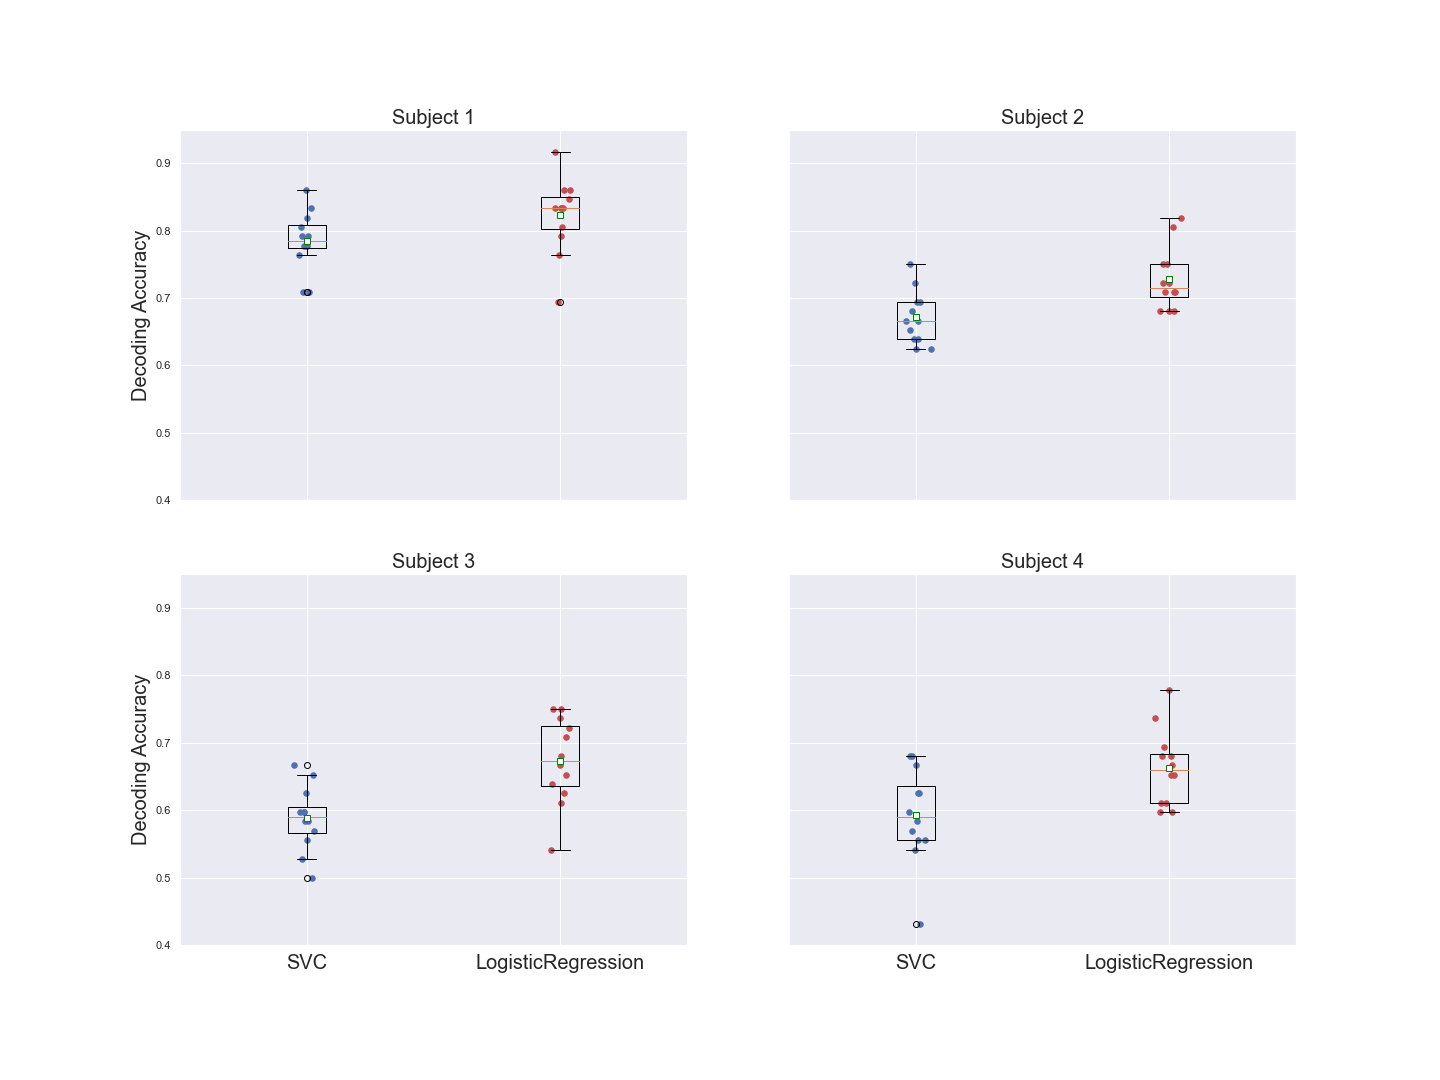
\includegraphics[width=\linewidth, height = 6cm]{some_subplots.png}%\hfill
        \caption{Subject-wise Accuracy for inherent OVR}
        \label{fig:ind_acc}
    	%\includegraphics[width=.33\textwidth]{sj2.png}
    	%\\%[\smallskipamount]
    	%\includegraphics[width=.33\textwidth]{sj3.png}%\hfill
    	%\includegraphics[width=.33\textwidth]{sj4.png}
        \end{subfigure}
        \begin{subfigure}[b]{0.49\linewidth}
        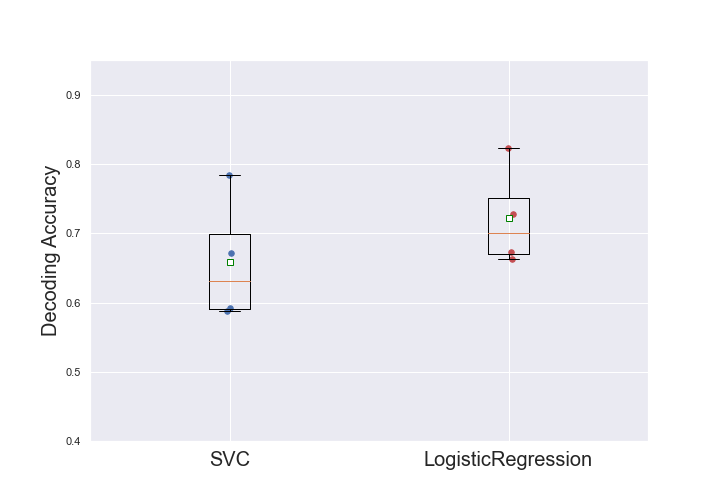
\includegraphics[width=\linewidth, height=6cm]{acc_tot_new.png}
        \caption{Total Accuracy for inherent OVR}
        \label{fig:tot_acc}
        \end{subfigure}
    \caption{Accuracy scores for the given multiclass strategies implemented. Green squares denote mean accuracy across participants (a,b,d) or folds (c) and filled colored circles denote the accuracy for individual participants (a,b,d) or scores from individual folds for the given participant (c). \textbf{(a)} Accuracy for OVO strategy (SVC: 55.93\%, LR: 54.57\%). \textbf{(b)} Accuracy for OVR strategy (SVC: 55.90\%, LR: 61.11\%). \textbf{(c)} Accuracy for individual subjects with the inherent OVR strategy (S1: 78.47\%, 82.29\%; S2: 67.13\%, 72.80\%; S3: 58.80\%, 67.36\%; S4: 59.26\%, 66.32\%; for SVC and LR, respectively). \textbf{(d)} Accuracy for inherent OVR strategy (SVC: 65.91\%, LR: 72.19\%).}
    \label{fig:all_acc}
\end{figure}

%\newline
%
\textbf{b)} In the same leave-one-run-out cross validation as in \textbf{a)}, the decoding accuracy of the individual categories was calculated. The mean percent true positives calculated across all folds and participants for the respective models are displayed in Figure \ref{fig:ind_cl} and reported in Table \ref{tab:cat_score}. Categories that were able to be decoded best were \textit{face, house}, and \textit{scrambledpix}. \textit{Bottle} and \textit{scissors} were the categories least able to be decoded.  

\begin{figure}[hbt!]
\centering
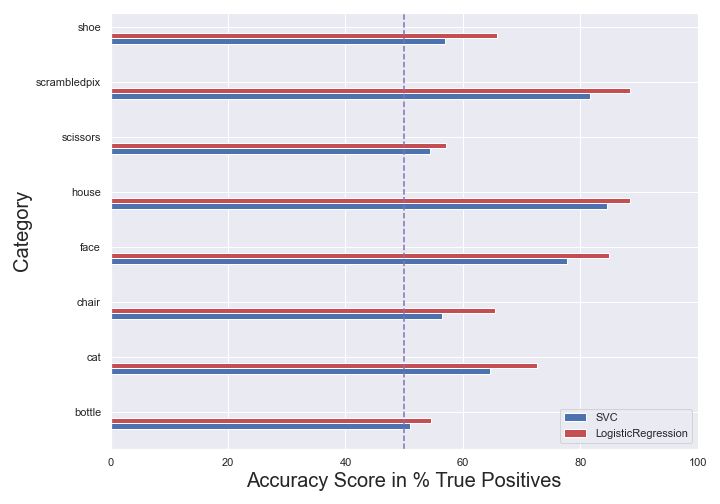
\includegraphics[width=0.85\textwidth]{ind_classes.png}
\caption{Mean decoding accuracy for individual categories (inherent OVR).}
\label{fig:ind_cl}
\end{figure}
%\newline
%\newline{}
\begin{table}[hbt!]
\centering
\caption{Accuracy scores for individual categories in \% for SVC and LR (inherent OVR).}
\begin{tabular}{||l||l|l|l|l|l|l|l|l||}
\cline{1-9}
Model  & \multicolumn{1}{l|}{shoe} & \multicolumn{1}{l|}{scr-pix} & \multicolumn{1}{l|}{scissors} & \multicolumn{1}{l|}{house} & \multicolumn{1}{l|}{face} & \multicolumn{1}{l|}{chair} & \multicolumn{1}{l|}{cat} & bottle \\ \hline \hline
SVC    & 56.94                     & 81.71                        & 54.40                         & 84.49                      & 77.77                     & 56.48                      & 64.58                    & 50.93  \\ %\cline{1-1}
LR & 65.74                     & 88.43                        & 57.18                         & 88.43                      & 84.95                     & 65.51                      & 72.69                    & 54.63  \\ \cline{1-9}
\end{tabular}
\label{tab:cat_score}
\end{table}
\textbf{c)} In a final step, the nested cross validation with a linear SVM and the inherent OVR strategy was set up using \verb|sklearn|'s \verb|GridSearchCV| function. The train data set was composed of runs 1-6 and 10-12, while the test data was the remaining runs 7-9, resulting in 75\% of the data being used for finding optimal hyperparameters in the cross validation and training the model and 25\% for the final model evaluation. The parameter space was searched for the best k features to retain from 1000 to 2000 in 5 steps of 250 and the best regularization parameter C in 8 exponential steps from $10^{-5}$ to $10^2$. The results are shown in Table \ref{tab:ncv}. Using these hyperparameters, the mean accuracy of the linear SVC across subjects (70.83\%) increases to a similar value as the LR in \textbf{a)}.

\begin{table}[hbt!]
\centering
\caption{Results from the nested cross validation with a linear SVC.}
\begin{tabular}{||l||c|c|c|c||}
\hline
Subject & Best C & Best k & \multicolumn{1}{l|}{Best CV Score {[}\%{]}} & \multicolumn{1}{l||}{Test Set Score {[}\%{]}} \\ \hline \hline
1       & 0.001  & 2000   & 77.93                                       & 83.33                                        \\ \hline
2       & 0.001  & 1000   & 72.07                                       & 72.69                                        \\ \hline
3       & 0.001  & 1000   & 68.06                                       & 62.50                                        \\ \hline
4       & 0.001  & 1000   & 59.88                                       & 64.81                                        \\ \hline
\end{tabular}
\label{tab:ncv}
\end{table}
\break
A subsequent nested cross validation using a LR model with the inherent OVR strategy and the same settings as above was performed to check if the accuracy would improve for this model as well after finding optimal hyperparameters. Surprisingly, the mean accuracy of the LR model actually decreased when using this cross validation scheme (67.59\%). The results are shown in Table \ref{tab:cv_lr}. Interestingly, while the leave-one-run-out cross validation shows the LR performing better, using nested cross validation the linear SVC performs slightly better than the LR. This might be due to the fact that we only have one test set where we evaluate the accuracy of the model on. Performing a nested cross validation with different subsets of the data defined as training and test sets would be a potential next step to see whether these results are artefactual or, since the leave-one-run-out cross validation is trained on $\frac{11}{12}$ of the data, the LR benefits from a greater amount of training data. Similarly, performing another leave-one-run-out cross validation with the parameters found for the linear SVC might clarify if the model performs similarly in that setting with the greater amount of training data or performs better when trained on less data (as in the nested cross validation), in the sense that this might additionally reduce the likelihood of overfitting.

\begin{table}[hbt!]
\centering
\caption{Results from the nested cross validation using LR.}
\begin{tabular}{||l||c|c|c|c||}
\hline
Subject & Best C & Best k & \multicolumn{1}{l|}{Best CV Score {[}\%{]}} & \multicolumn{1}{l||}{Test Set Score {[}\%{]}} \\ \hline \hline
1       & 1.0  & 1500   & 79.01                                       & 79.63                                        \\ \hline
2       & 1.0  & 1000   & 70.22                                       & 67.59                                        \\ \hline
3       & 0.01  & 1250   & 68.21                                       & 62.04                                        \\ \hline
4       & 0.01  & 1250   & 61.27                                       & 61.11                                        \\ \hline
\end{tabular}
\label{tab:cv_lr}
\end{table}

\break
\clearpage
\section*{\centering \underline{Problem 2}}

For the error function 
\begin{eqnarray}
E(w) = E_D(w) + \lambda E_W(w)
\label{eq:complete_err}
\end{eqnarray}
with
\begin{eqnarray}
E_D(w) = \frac{1}{2}\sum^N_{n=1} (t_n - w^Tx_n)^2
\label{eq:RSS}
\end{eqnarray}
and
\begin{eqnarray}
E_W(w) = \frac{1}{2}\sum^M_{j=1}|w_j|^q 
\label{eq:reg}
\end{eqnarray}
$\lambda $ is the regularization coefficient that controls the magnitude of regularization, while $q$ defines the type of regularizer of the error function. \newline

For illustrating the behavior of the error function (\ref{eq:complete_err}) as a function of $\lambda$ and $q$, we will look at a simple linear regression example. Assume we have the data points shown in Figure \ref{fig:lina}, which are a subset of a larger data set, and a regression line fit to these points. If we now want to predict some out-of-training data from that same data set as shown in Figure \ref{fig:linb} in cyan, there might be a different slope that additionally can account better for the variation in the new data similar to the regression line in cyan. In these cases, regularization can become helpful for finding weights that increase the performance of a model on out-of-training data. Fitting the model too strictly to the training data -- especially with high dimensional data -- oftentimes leads to overfitting, so regularization is one method of counteracting this.
\begin{figure}[h]
	\centering
    \begin{subfigure}[b]{0.49\linewidth}
        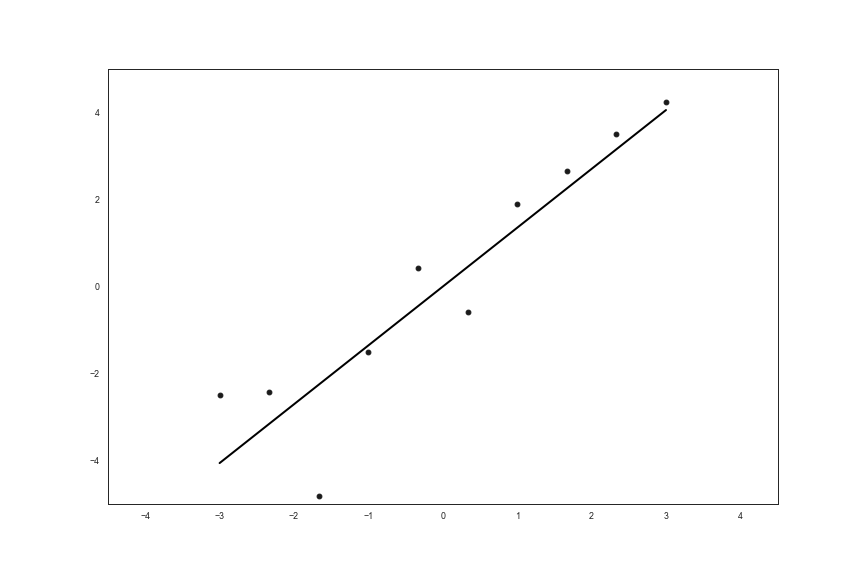
\includegraphics[width=\linewidth]{lina.png}%\hfill
        \caption{Some data with a regression line fit to it.\newline}
        \label{fig:lina}
    \end{subfigure}
    \begin{subfigure}[b]{0.49\linewidth}
        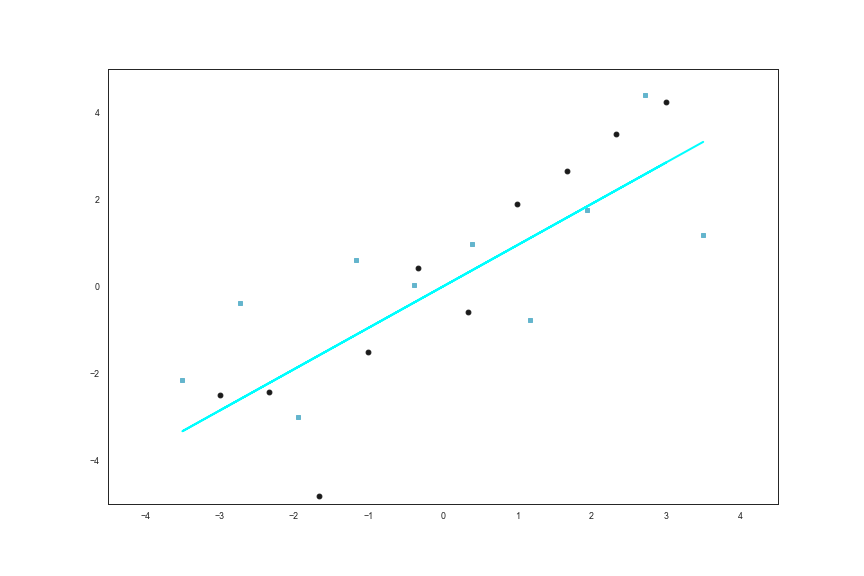
\includegraphics[width=\linewidth]{linb.png}%\hfill
        \caption{Including out-of-training data indicates that there might be a different optimal regression line.}
        \label{fig:linb}
    \end{subfigure}
    \label{fig:slr}
    \caption{Sample data for a simple linear regression.}
\end{figure}
\\
Taking a first look at equation (\ref{eq:complete_err}), we can see that when $\lambda = 0$, this is equivalent to an error function only consisting of the residual sum of squares (eq. \ref{eq:RSS}). Increasing $\lambda$ results in a higher penalization of the weights and, therefore, smaller values will be favored in order to minimize the error function (see Figure \ref{fig:lambda}). In our simple linear regression example, higher $\lambda$ values lead to a less steep slope of the model, indicated by the filled colored circles in Figure \ref{fig:lasso} and \ref{fig:ridge} that denote the slope which leads to the lowest value of the error function given a specific value of $\lambda$. One of the slopes fit to the training data with a specific $\lambda$ value should then be able to account for the out-of-training data better.

In addition, we can see how different $q$ values influence the regularization. In Figure \ref{fig:lasso} we see the behavior with $q=1$ (l1 or lasso regularization) on our sample data from above, which shows that increasing $\lambda$ eventually leads to an optimal slope of $0$. Regularization with l1 can be very useful when a dataset contains a large amount of features, as it effectively reduces the dimensionality of the data to only keep those weights that were initially high and important as it shrinks large and small values equally, resulting in a sparse array of weights. On the other hand, Figure \ref{fig:ridge} shows the behavior for $q=2$ (l2 or ridge regularization). Due to its quadratic term, l2 regularization does not shrink weights fully to $0$ and, therefore, does not effectively reduce dimensionality, however it penalizes higher weights more strongly because of it. This means that larger weights are shrunken more strongly with an l2 regularizer in comparison to l1 (steeper curves on the right in \ref{fig:ridge}). Optimally, this leads to a change in bias of the model so that it can be better generalized to out-of-training data and is more robust to features obscuring the results, meaning it reduces the out-of-training error in the long run by forgoing an optimal fit to the training data. Increasing $q$ further leads to penalties that effect larger weights even heavier. Taken together, both l1 and l2 (and $q>2$) penalties reduce model complexity and with that counteract overfitting, however have different effects on the weights of a model that need be taken into account, depending on what the goal of the model should be, i.e. are we looking for a sparse solution where all weights are penalized the same, then consider l1, or are we looking for a solution that penalizes greater weights more heavily, then consider l2. 
\begin{figure}[htb!]
	\centering
    \begin{subfigure}[b]{0.8\linewidth}
        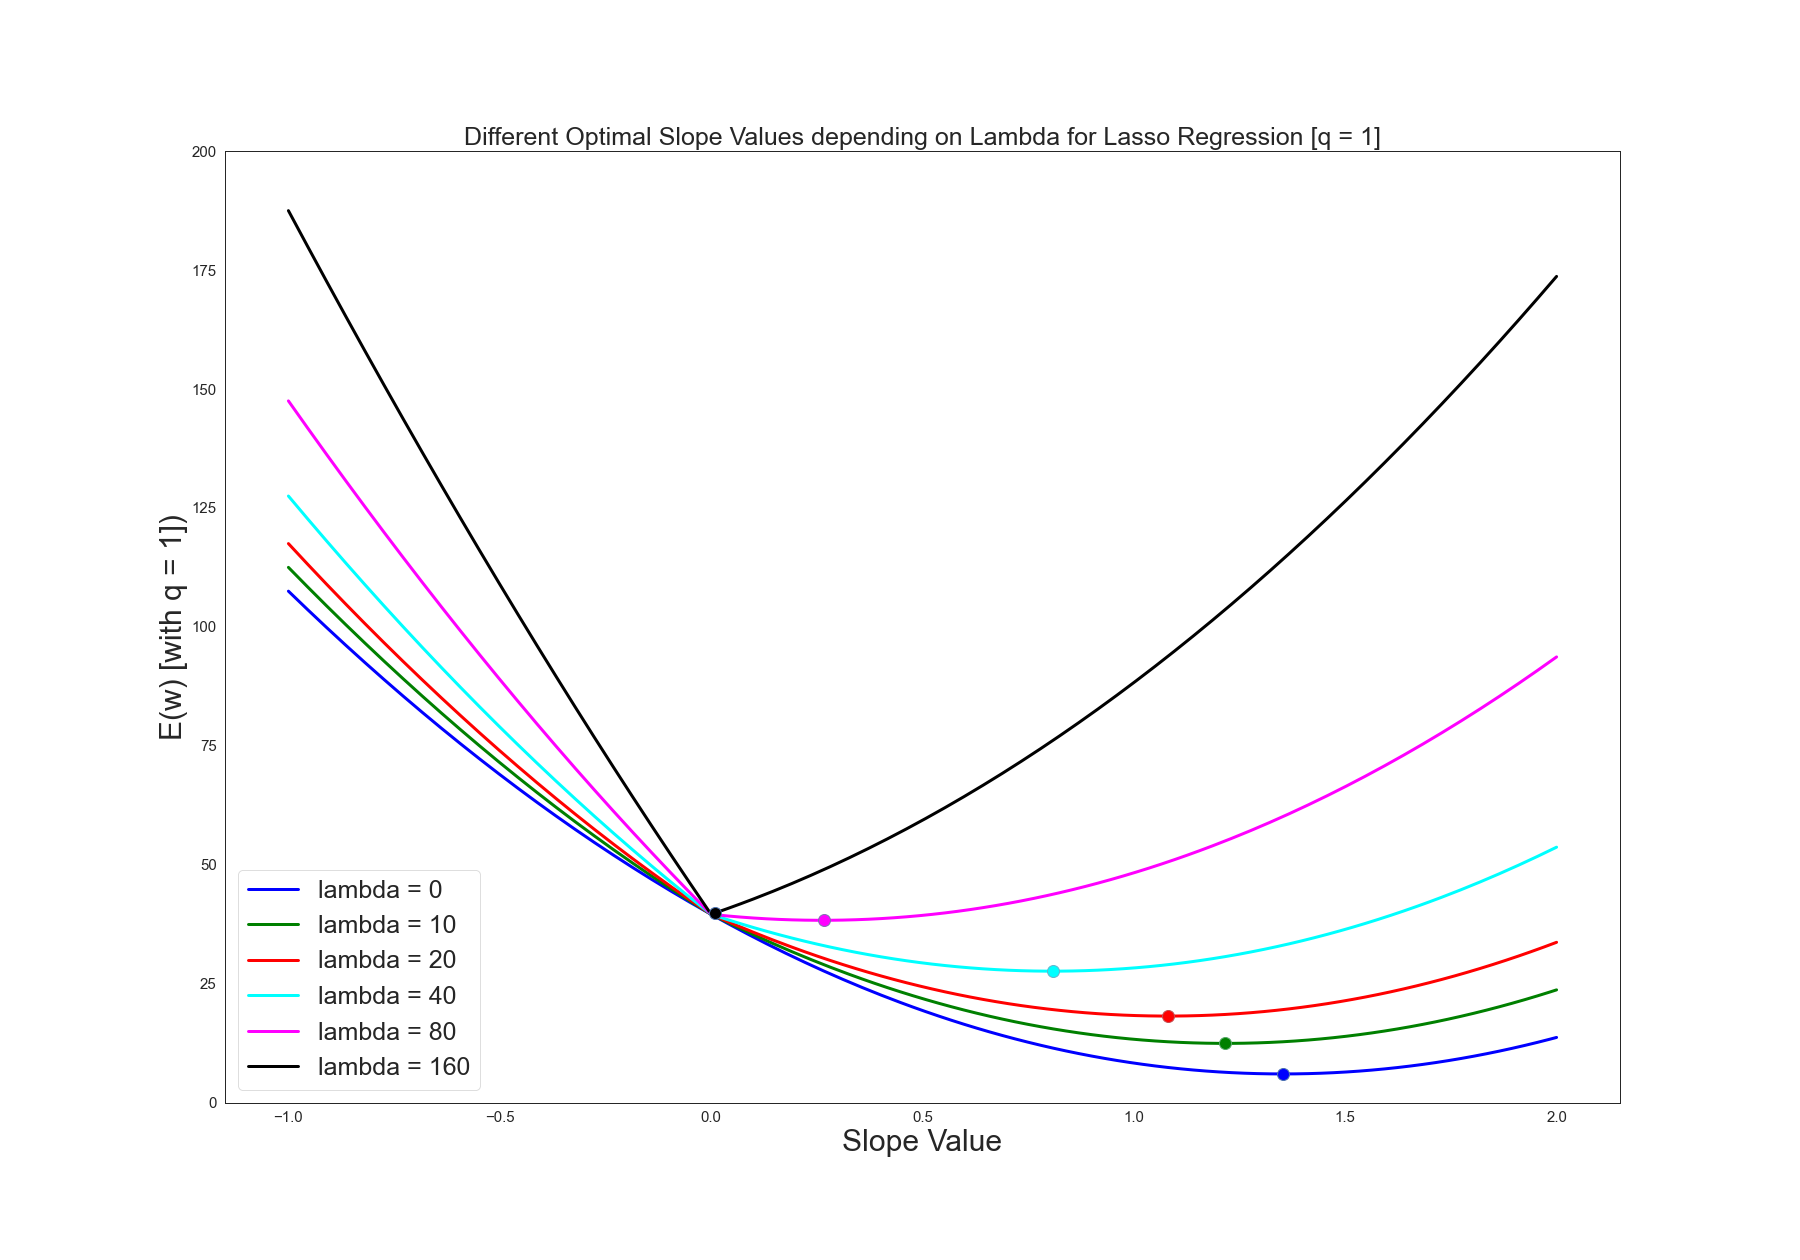
\includegraphics[width=\linewidth]{lasso.png}
        \caption{Change in optimal slope values as a function of $\lambda$ for Lasso Regression [$q = 1$].}
        \label{fig:lasso}
    \end{subfigure}
    \begin{subfigure}[b]{0.8\linewidth}
        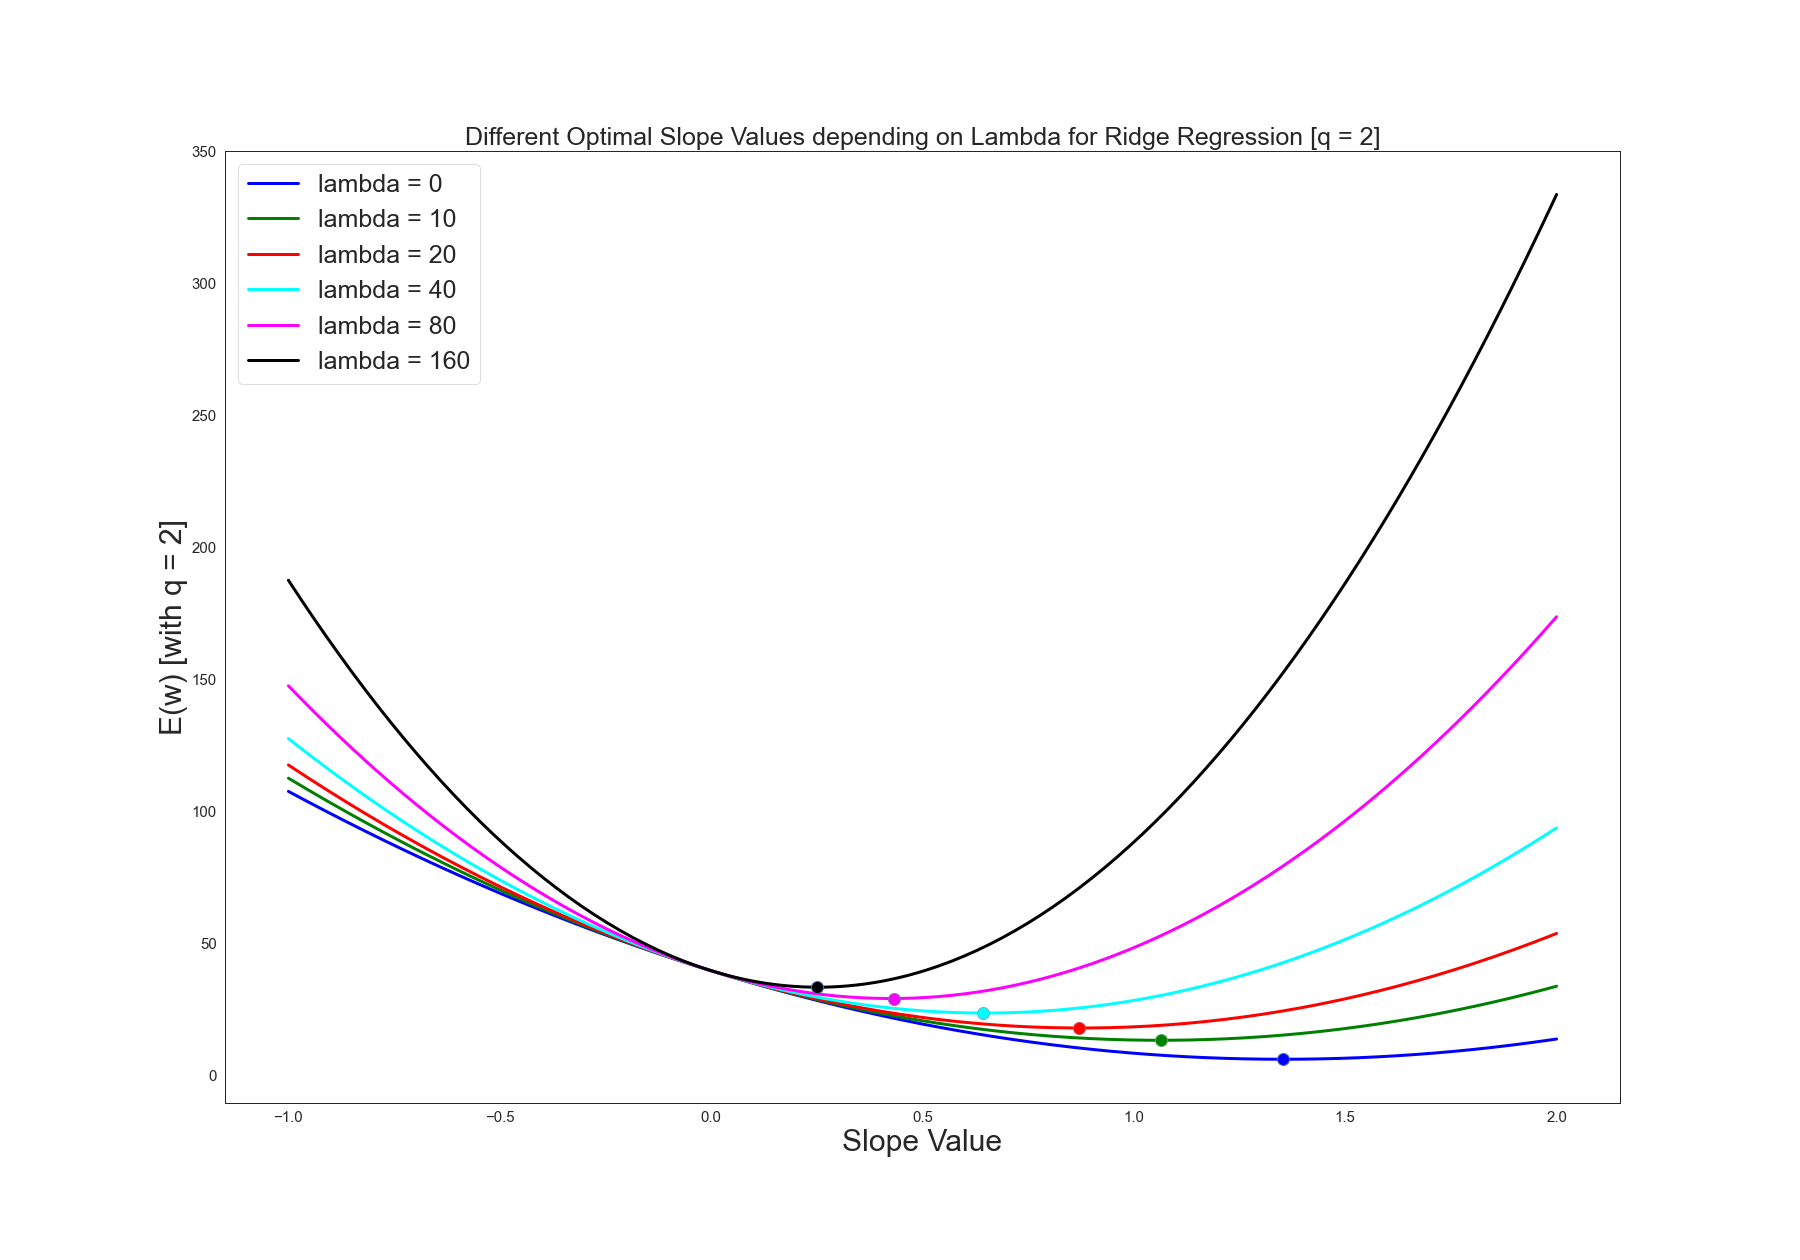
\includegraphics[width=\linewidth]{ridge.png}
        \caption{Change in optimal slope values as a function of $\lambda$ for Ridge Regression [$q = 2$].}
        \label{fig:ridge}
    \end{subfigure}
    \caption{Behavior of $E(w)$ as a function of $\lambda$ and $q$ for the data in Figure \ref{fig:lina}. Filled colored circles denote minimum of the error function and, therefore, the optimal slope value for the given $\lambda$ value.}
    \label{fig:lambda}
\end{figure}


\end{document}
